%%%%%%%%%%%%%%%%%%%%%%% file template.tex %%%%%%%%%%%%%%%%%%%%%%%%%
%
% This is a general template file for the LaTeX package SVJour3
% for Springer journals.          Springer Heidelberg 2010/09/16
%
% Copy it to a new file with a new name and use it as the basis
% for your article. Delete % signs as needed.
%
% This template includes a few options for different layouts and
% content for various journals. Please consult a previous issue of
% your journal as needed.
%
%%%%%%%%%%%%%%%%%%%%%%%%%%%%%%%%%%%%%%%%%%%%%%%%%%%%%%%%%%%%%%%%%%%
%
% First comes an example EPS file -- just ignore it and
% proceed on the \documentclass line
% your LaTeX will extract the file if required
%
\RequirePackage{fix-cm}
%
%\documentclass{svjour3}                     % onecolumn (standard format)
%\documentclass[smallcondensed]{svjour3}     % onecolumn (ditto)
\documentclass[smallextended]{svjour3}       % onecolumn (second format)
%\documentclass[twocolumn]{svjour3}          % twocolumn
%
\smartqed  % flush right qed marks, e.g. at end of proof
%
\usepackage{graphicx}
%
% \usepackage{mathptmx}      % use Times fonts if available on your TeX system
%
% insert here the call for the packages your document requires
%\usepackage{latexsym}
% etc.
\usepackage{gensymb}
\usepackage{colortbl}

%
% please place your own definitions here and don't use \def but
% \newcommand{}{}
\newcommand{\FIXME}[1]{\textcolor{red}{FIXME: #1}}

%
% Insert the name of "your journal" with
% \journalname{myjournal}
%
\begin{document}

\title{Water in the Cloud: Understanding Water Chemistry via the
Internet of Things\thanks{This paper builds on the previously published work,
Roger D. Chamberlain, Mike Chambers, Darren Greenwalt, Brett Steinbrueck,
and Todd Steinbrueck, ``Water in the Cloud: Remote Understanding of Water
Chemistry: Poster Abstract,'' in Proc.~of ACM/IEEE 2nd International
Conference on Internet-of-Things Design and Implementation (IoTDI),
April 2017, pp. 353-354. DOI: 10.1145/3054977.3057327}
}
%\subtitle{Do you have a subtitle?\\ If so, write it here}

\titlerunning{Water in the Cloud}        % if too long for running head

\author{Roger D. Chamberlain
\and
 Mike~Chambers
\and
 Darren~Greenwalt
\and
 Brett~Steinbrueck
\and
 Todd~Steinbrueck
}

\authorrunning{R.D. Chamberlain et al.} % if too long for running head

\institute{R.D. Chamberlain \at
              Washington University in St. Louis %\\
              and BECS Technology, Inc., St. Louis, MO USA \\
              \email{roger@wustl.edu}
           \and
           M. Chambers $\cdot$ D. Greewalt $\cdot$ B. Steinbrueck $\cdot$ T. Steinbrueck \at
              BECS Technology, Inc., St. Louis, MO USA
           \and
           M. Chambers \at
              \email{mike\_c@becs.com}
           \and
           D. Greenwalt \at
              \email{darren@becs.com}
           \and
           B. Steinbrueck \at
              \email{brett@becs.com}
           \and
           T. Steinbrueck \at
              \email{todd@becs.com}
}

\date{Received: date / Accepted: date}
% The correct dates will be entered by the editor


\maketitle

\begin{abstract}
Water treatment is one of those essential elements of modern life
that is taken for granted by the general population.
We describe the ability to remotely understand and
improve water chemistry using IoT devices attached to the cloud.
The commercial benefits of this IoT connectivity are substantial,
including: reduced chemical usage, improved chemical inventory 
management, safer operation (fewer and less critical alarms),
reduced maintenance costs, and higher quality water.

\keywords{IoT \and Water chemistry}
% \PACS{PACS code1 \and PACS code2 \and more}
% \subclass{MSC code1 \and MSC code2 \and more}
\end{abstract}

\section{Introduction}
\label{sec:intro}

The Internet of Things (IoT) provides tremendous opportunities for
enhanced quality of life; however, the realization of these opportunities
requires both the technical ability to deliver them and the economic
incentives to provide them.
Clean water is a benefit to all, and generally is taken for granted
by the citizenry of the industrialized world.
Yet, \FIXME{talk about challenges and how IoT can make it better.}

BECS Technology, Inc., is a firm that provides water chemistry monitoring
and control equipment to the aquatics market, which includes a number
of (mostly distinct) market segments (e.g., pools, including municipal pools,
commercial pools, water parks, health clubs, animal habitats in zoos,
residential pools; drinking water treatment facilities; waste water
treatment facilities; fountains; building cooling towers; irrigation
systems; and various commercial operations, including washing vegetables,
fracking; etc.).
Its BECSys\texttrademark{} line of controllers measure
a number of aspects of water chemistry (e.g., pH,
oxidation-reduction potential (ORP), free chlorine concentration,
temperature, conductivity, turbidity, alkalinity~\cite{cew18},
etc.) and perform various control operations (e.g., feed chemical)
to ensure that the water chemistry stays within desired parameters.

EZConnect\texttrademark{}
is the security infrastructure BECS has developed to provide
remote access capability to equipment it manufactures.  This remote
access capability satisfies the need for security yet balances
that need with the equivalent need for ease of installation and
maintenance~\cite{ezconnect,ccgss18}.

Here, we describe EZAnalytics\texttrademark{}, the use of the EZConnect infrastructure to enable
cloud-based data logging and analytics on water chemistry data from a
collection of controllers.

\FIXME{Introduce e-commerce angle.
Ease of use is important in e-commerce~\cite{gefen2000}.}

\section{Background and Related Work}
\label{sec:background}

BECS Technology's controllers are fairly typical devices
in the Internet of Things (IoT).
The controller itself monitors various aspects of water chemistry
and, based on these readings, takes various actions
(feeding chemical, adjusting recirculation flow rate, etc.) to maintain
the water chemistry within desired parameters.
Alarm conditions trigger notifications to service personnel.
Sensor values and actions are all logged internally,
and these logs are frequently used when diagnosing the causes
of alarms or other anomalous events.
Remote access to all of the above information is
clearly to the benefit of the equipment owners/operators.

Figure~\ref{ezconnect} shows the essential components of the EZConnect
system.
Water chemistry controllers are typically installed on a local-area network
behind a firewall.
Applications (either desktop programs or mobile apps) wish to communicate
with the controller.  Since the firewall (correctly) blocks incoming
communications requests, data transfer is facilitated by the controller
making an outbound connection to the EZConnect server, which accepts
requests for communication to a controller, validates the authority to do
so, and forwards vetted messages to/from the controller.

\begin{figure}[htbp]
 \center
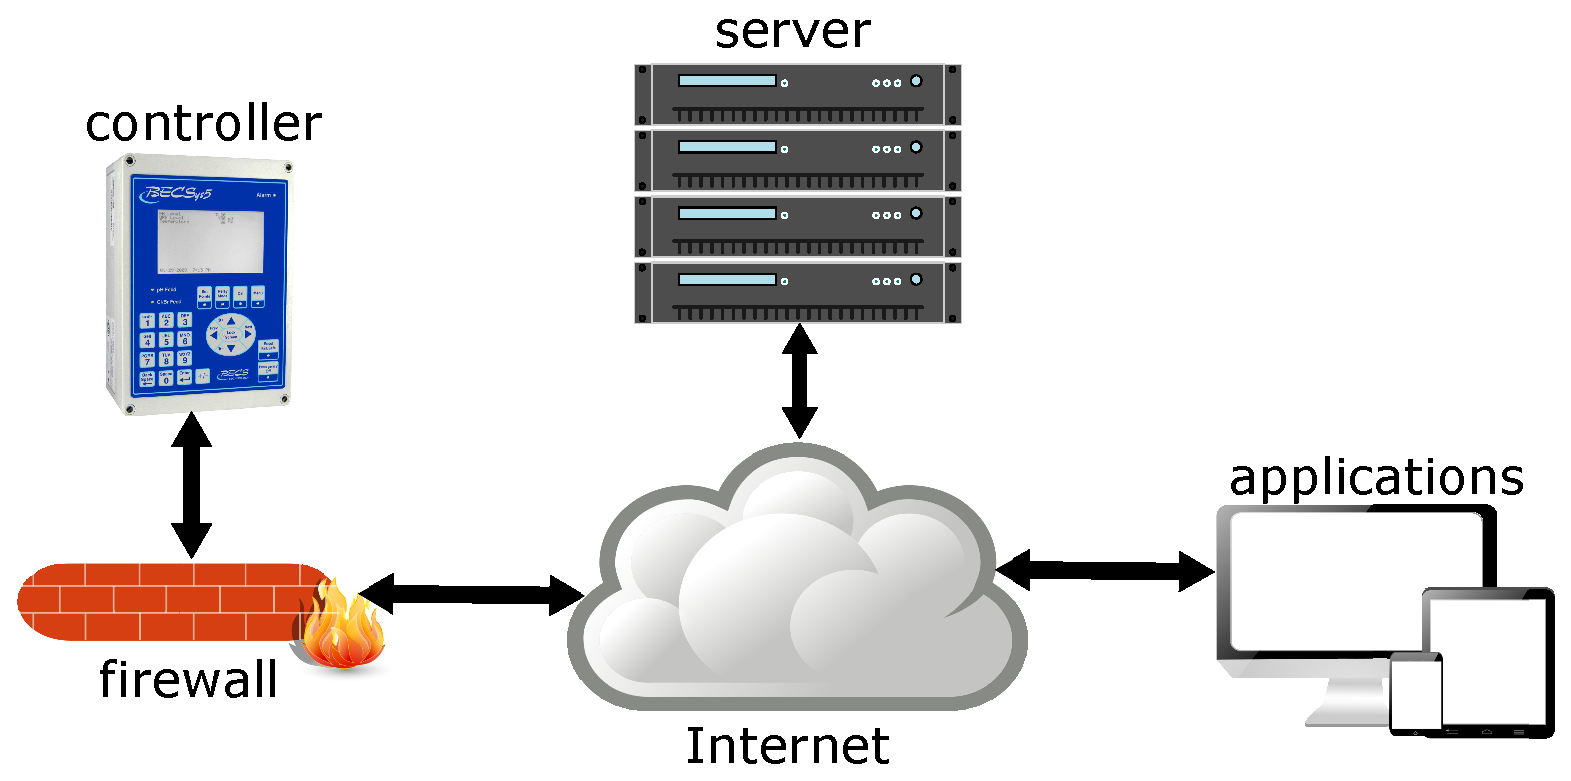
\includegraphics[width=\columnwidth]{EZConnect}
    \caption{EZConnect system diagram~\protect\cite{ezconnect}. The controller
opens a connection to the server in the cloud, which then facilitates communication with the controller by desktop programs or mobile apps.}
    \label{ezconnect}
\end{figure}

Remote capabilities include viewing of current status, downloading
of data logs, and configuration of the controller.
Figure~\ref{console} illustrates a realtime view of water chemistry
for a specific body of water
as remotely displayed on a PC screen.  Four readings are being shown:
pH (at\,7.1), ORP (at 750\,mV), temperature (at 83\,\degree F), and
free chlorine (at 1.0\,ppm).  Also indicated are the set points and
high and low alarm points for each reading as well as the control
outputs (in this example control is based on pH and ORP).
The two dials at the bottom show a pair of indices
(Langelier Saturation Index and Ryznar Stability Index)
which are indicators of the scaling properties of the water~\cite{mb88}.
The panel on the left allows the user to navigate to different
controllers (either at the same or a different physical location).
The tabs at the top allow the user to access a menu tree that
can examine and/or modify a multitude of parameters on the controller.

\begin{figure}[ht]
 \center
\includegraphics[width=0.9\columnwidth]{console}
    \caption{Console display of controller at remote location~\protect\cite{ccgss18}.}
    \label{console}
\end{figure}

Figure~\ref{graph} illustrates data logs collected over a 2 day period.
The same four readings are plotted on the top graph, and the bottom
graph gives indications of control actions, alarms, and other events.
In the top curve, one can readily see disturbances in the pH at noon
on both days.
The additional window on the right shows the instantaneous values
at the position of the cursor (the vertical line positioned
by the user at 9am on the first day).
As above, the leftmost panel supports navigation to different
controllers.

\begin{figure}[ht]
 \center
\includegraphics[width=1.0\columnwidth]{graph}
    \caption{Plot of controller data logs~\protect\cite{ccgss18}.}
    \label{graph}
\end{figure}

In addition to diagnosing the root causes of errors in the water
chemistry, the historical logs also enable the tracking of
parameter changes by operators as well as support the demonstration
and documentation of regulatory compliance.

The security of these controllers is
state-of-the-art~\cite{ezconnect,ccgss18}, with special attention given
to ease-of-use considerations, as there is ample evidence that
security measures that are difficult to implement are frequently
circumvented by users~\cite{gefen2000,hertzum2004,schneier16}.
Schneider~\cite{schneier16} cautions us all that security must
not rely on unreasonable expectations about the actions of users.
``We must stop trying to fix the user to achieve security.''
To be truly effective, any approach to security must be paired
with an approach to ease the burden on the user~\cite{gefen2000}.
Hertzum et al.~\cite{hertzum2004} assessed the intrinsic tensions between
security and ease of use in an e-banking context, and concluded
that ease of use limitations can directly contribute to decreased
security.

We must not sacrifice true security, however, in the name of ease
of use.  We need both, especially given the fact that
the security of IoT devices has been shown to be particularly
vulnerable, Cui and Stolfo~\cite{cs11} and Costin et al.~\cite{Costin2014}
have identified significant numbers of IoT devices
(over a million) with exposed vulnerabilities.

There has been significant work in the area of IoT and how it relates
to e-commerce.
Klock et al.~\cite{kpm11} describe the necessary infrastructure,
business possibilities, and barriers for e-commerce to thrive, particularly
as it relates to small- and medium-size enterprises.
Glova et al.~\cite{gsv14} analyze business models for the IoT environment,
reducing the business activity to its core elements, ``the value proposition,
distribution channels and the customers.''
Zhang and Wen~\cite{zw17} propose the use of blockchain technology in IoT
e-business,
and Xu~\cite{Xu14} reviews the development trends of IoT applications
in e-commerce.

Specific examples of IoT-based e-commerce include the following.
A decade ago,
Wamba et al.~\cite{wlbl08} assessed RFID technology's use in 
business-to-business e-commerce with a case study in the retail sector.
More recently,
Bi et al.~\cite{bxw14} described the impact of IoT on manufacturing, in
part driven by e-commerce.
Ruan and Shi~\cite{rs16} proposed an approach to monitoring the
freshness of fruit in-transit, and
Yu et al.~\cite{ywzh16} reviewed the state-of-the-art in
e-commerce logistics for supply chain management.

\section{Data to the Cloud}
\label{sec:cloud}

There is a significant amount of data that is currently retained by
the controllers about water chemistry.  This includes historical
information on sensor readings (e.g., pH, oxidation-reduction potential (ORP),
free chlorine concentration, temperature, conductivity, turbidity,
alkalinity, etc.),
alarms (e.g., readings out of range, etc.), and user actions (e.g.,
set-point changes, etc.).
In addition, information on chemical stocks are frequently monitored
and logged as well.

It is currently possible to retrieve all of the above information from
a controller to a desktop application or mobile app by connecting to
the EZConnect server, providing appropriate authentication, and asking
the controller for its internal data logs.

Our current endeavor is
to collect this information off of a collection of controllers (e.g., all
owned by an individual organization), retain the collected data in
the cloud, and realize benefit from the aggregation that is not realized
from each individual controller's data in isolation.

Owner/operators of this equipment are responsible for 
more than one controller, and they would benefit significantly from a relevant
summary view of the state of the water chemistry under their purview.
An example of a summary view (appropriate for each controlled body of water)
is illustrated in Figure~\ref{screenshot}.

\begin{figure}[htbp]
 \center
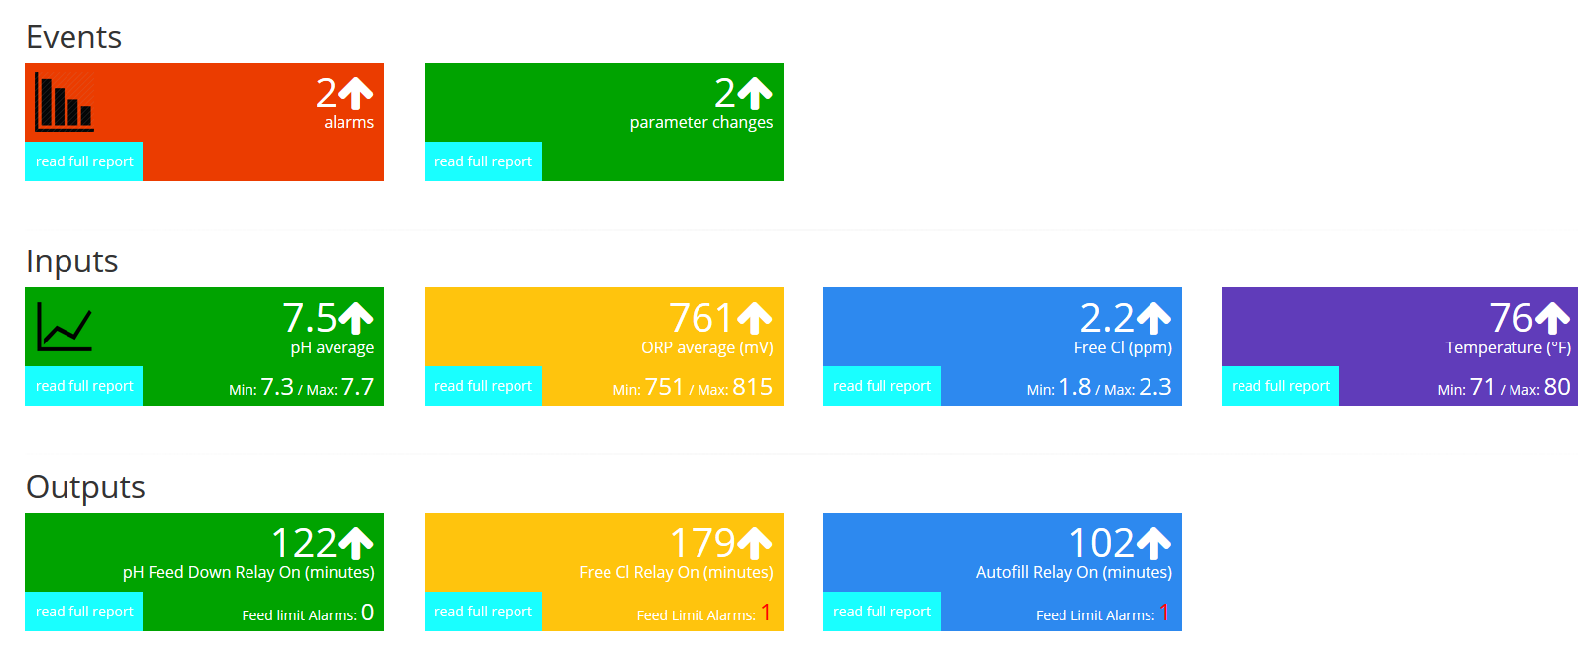
\includegraphics[width=\columnwidth]{screenshot}
    \caption{Screen capture of summary view data presentation. Additional
details are available via a link associated with each individual item.}
    \label{screenshot}
\end{figure}

In the figure, relevant information is organized for quick reference,
highlighting the ``big picture'' of the water chemistry, and allowing for
a more detailed drill down via a link associated with each item.
Groups of items are organized into categories (e.g., events, inputs,
outputs), and current values are supplemented with trends (indicated
by directional arrows) and ranges of values for the previous time period.

The above is facilitated by a number of concurrent processes running
in the EZConnect server (which is deployed in the cloud).  First,
a data logging process periodically communicates with each connected
controller and retrieves the data logs for that immediate past period.
Second, those data are inserted into a persistent database.  Third,
a report generator mines the database to generate the information needed
for the summary view, and finally, the summary view is served to the
user via a secure web server.

\section{Data Analytics}
\label{sec:analytics}

While the summary data presentation is valuable to users, particularly for
understanding the current state of the water chemistry that is immediately
their responsibility, the true value of the data in the cloud is what it
can potentially tell us about water treatment generally, and the impact
that it can have commercially.
By combining data from a number of controllers, we can learn more than
it is possible to discern from any one example.

We are aggregating controller data in two ways.  First, data that are
from controllers all owned by an individual organization can be readily
combined and mined for the benefit of that organization.  They own
both the equipment and the data. Second, for those organizations that
give permission, anonymized data sets can be made available for mining
(e.g., see~\cite{horey2007,zhong2009k}), providing for a potentially
much larger data set.

There are a number of things we hope to learn from these data.
\begin{itemize}
\item The effectiveness of control decisions.  How well do different
approaches work at maintaining water chemistry control?  What factors
are important?
\item How to recommend better control approaches.  How well will control
approaches that are effective in one body of water transfer to another?
\item How to minimize chemical usage.  The data logs not only contain
sensor readings of water chemistry, but also log chemical feed rates
and supplies.  Can we make water chemistry control more cost effective,
by decreasing the consumables needed?
\item How to predict problems. Alarm conditions (e.g., due to water
chemistry being out of balance) require fast and expensive human response.
Both public safety and maintenance effort required will be improved
if we can predict problems prior to them reaching the level of an alarm.
\end{itemize}

Modern machine learning techniques are well suited to addressing the
questions we pose above.
While the data analysis has not yet happened, as the system is just
now being deployed in the field, we are very optimistic that new insights
will come from the data aggregation described above.

The first example of commercial impact is on inventory monitoring
and resupply. It is frequently the case that chemical inventories
are monitored by the controllers, which can straightforwardly enable
automated re-ordering of chemical as well as scheduling of delivery.
Not only does this reduce the manual workload associated with
inventory control, it also reduces cases of inadvertent supply outages
which can result in anomalous water chemistry.

The second example is a significant reduction in maintenance costs
for operators.  By alerting operators to potential
issues with the water chemistry before it reaches alarm levels, 
the organization can be much more flexible in scheduling service
personnel. E.g., an operator can investigate the issue remotely,
querying the controller for relevant information; the need for
a dispatch to the physical site might not need to be an emergency, but can
instead by folded into a more convenient schedule; and when the
issue can be resolved in time, an alarm condition can be averted.

The above two examples are cases where the data of interest is specific
to the bodies of water (and associated controllers) that are the
responsibility of an individual organization.  Tossing our net
even wider, by aggregating data from disparate organizations, it
is possible to gain even more benefit.

As an example of benefits gained by data aggregation, improved
control techniques can be more widely disseminated and used.
In the context of recreational water, a million gallon competition
pool doesn't react in the same way as a lazy river, or a shallow
splash pool designed for the very young. Data aggregation across
organizations allows for operators to see the effects of control
techniques on each of these bodies of water separately, yet with
sufficient examples of each type that general conclusions can
reasonably be drawn.

These control techniques might be simple things, such as parameter
settings in the existing control algorithms, or they might be
more involved, such as more sophisticated control algorithms
(e.g., under what conditions time proportional control~\cite{McP13}
is beneficial). The overall goal, however, is the same in each
case. We want to improve water quality control by improved techniques
driven by data analysis across multiple sites and organizations.

The e-commerce implications of this can be significant, with the
primary benefits being reduced chemical usage and reduced maintenance
costs (due to fewer issues that need to be addressed).

The above can all be accomplished while preserving the confidentiality
of the data associated with specific sites.  There are a number
of robust techniques now available for sharing aggregate data
while maintaining originators' anonymity~\cite{horey2007,zhong2009k}.

\section{Conclusions and Future Work}
\label{sec:conclude}

EZAnalytics provides an operational ability to collect water chemistry
data from a collection of control equipment.  This data collection
is secure, and supports multiple levels of data analysis.
The initial deployment provides summary data to equipment owners/operators
about the water chemistry under their direct control.
This has direct implications for inventory management as well as
reduction in maintenance expenses.

The promise, however, is potentially substantially more beneficial.  We will
be able to use data from multiple installations to learn broad truths
about water chemistry control that can be shared across the industry.
This will result in lower chemical usage, fewer erroneous or alarm
conditions, and overall better control over water chemistry.


\section*{Conflict of Interest Statement}
On behalf of all authors, the corresponding author states that there is no conflict of interest.

%\begin{acknowledgements}
%If you'd like to thank anyone, place your comments here
%and remove the percent signs.
%\end{acknowledgements}

% BibTeX users please use one of
%\bibliographystyle{spbasic}      % basic style, author-year citations
\bibliographystyle{spmpsci}      % mathematics and physical sciences
%\bibliographystyle{spphys}       % APS-like style for physics
\bibliography{paper}   % name your BibTeX data base


\end{document}
% end of file template.tex

